\begin{frame}
  \frametitle{The macroscopic approach irradiates a sample physically}
  The delayed neutron count rate is directly measured after sample irradiation.

  \begin{figure}[htbp!]
    \begin{center}
      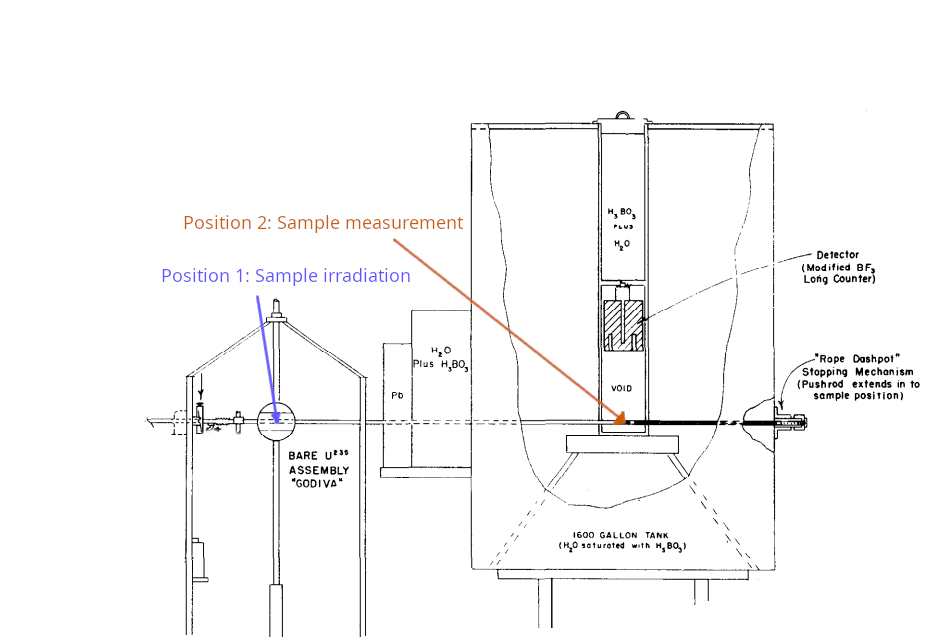
\includegraphics[width=0.6\textwidth]{../images/keepin-setup-mod.png}
    \end{center}
    \caption{Simplified experimental setup for measuring delayed neutron emission from irradiation of a 3 gram sample in Godiva referenced from \cite{keepin1957delayed}.}
    \label{fig:keepin-setup}
  \end{figure}
\end{frame}